%%%%%%%%%%%%%%%%%%%%%%%%%%%%%%%%%%%%%%%%%%%%%%%%%%%%%%%%%%%%%%%%%%%%%%%%%%%%%%%%
%2345678901234567890123456789012345678901234567890123456789012345678901234567890
%        1         2         3         4         5         6         7         8

\documentclass[letterpaper, 10 pt, conference]{ieeeconf}

\usepackage{setspace}\onespacing

%\documentclass[a4paper, 10pt, conference]{ieeeconf}      % Use this line for a4 paper

\overrideIEEEmargins                                      % Needed to meet printer 																			requirements.

%In case you encounter the following error:
%Error 1010 The PDF file may be corrupt (unable to open PDF file) OR
%Error 1000 An error occurred while parsing a contents stream. Unable to analyze the PDF file.
%This is a known problem with pdfLaTeX conversion filter. The file cannot be opened with Acrobat Reader.
%Please use one of the alternatives below to circumvent this error by uncommenting one or the other.
%\pdfobjcompresslevel=0
%\pdfminorversion=4

% See the \addtolength command later in the file to balance the column lengths
% on the last page of the document

% The following packages can be found on http:\\www.ctan.org
\usepackage{graphics} % for pdf, bitmapped graphics files
\usepackage{graphicx}
\usepackage{epsfig}   % for postscript graphics files
\usepackage{mathptmx} % assumes new font selection scheme installed
\usepackage{times}    % assumes new font selection scheme installed
\usepackage{amsmath}  % assumes amsmath package installed
\usepackage{amssymb}  % assumes amsymb package installed
\usepackage{physics}
\usepackage{caption}
\usepackage[font={small,it}]{caption}

% Added by Felix Fiedler
\usepackage{algorithm}		% http://ctan.org/pkg/algorithms
\usepackage{algpseudocode}	% http://ctan.org/pkg/algorithmicx
\usepackage{siunitx}
\usepackage{import} 		% for pdf_tex graphics
\usepackage{fixltx2e}

\newtheorem{assumption}{\textbf{Assumption}}
\newtheorem{lemma}{\textbf{Lemma}}
\newtheorem{theorem}{\textbf{Theorem}}

\title{\LARGE \bf
Case Study: PDE-Based Motion Planning for Robots
}
\author{ \textbf{Mehmet Batu Özmeteler} \\
\institute{Technische Universität Dortmund, Germany}}

\pagestyle{empty}

\begin{document}

\maketitle

%%%%%%%%%%%%%%%%%%%%%%%%%%%%%%%%%%%%%%%%%%%%%%%%%%%%%%%%%%%%%%%%%%%%%%%%%%%%%%%%
\begin{abstract}

This case study aims to utilize a proposed novel method for motion planning to implement
a canonical example for robots. The guiding approach for this work tackles the motion planning 
problem for systems with holonomic and non-holonomic constraints by building the method upon a  parabolic PDE that arises in the study of Riemannian manifold. The underlying method defines a metric for an optimal path, initializes a trajectory which connects the start and the end point (which doesn't have to respect constraints), and deforms the initial track via a homotopy into an admissible trajectory by numerically solving a system of coupled PDEs. The controls enabling the motion can be retrieved simply from the admissible path which in turn is practically optimal. By adhering to this procedure, this study performs its application for the two-link planar arm with additional holonomic constraints on the motion trajectory. Results are illustrated along with the benchmark example to demonstrate the viability of the implementation.

\end{abstract}
%%%%%%%%%%%%%%%%%%%%%%%%%%%%%%%%%%%%%%%%%%%%%%%%%%%%%%%%%%%%%%%%%%%%%%%%%%%%%%%%

\section{\textbf{Introduction}}

\subsection{Motion Planning for Non-holonomic Systems}

The principal objective of motion planning is to compute a trajectory attained by a sequence of controls, which satisfies certain dynamic and obstacle avoidance constraints to achieve an admissible, collision-free motion of the system from the source to destination. For linear systems, the problem is unambiguous; explicit solutions that steer the system from start to end do exist. However for the non-linear case, the situation is way more complicated.

Before moving on to why, an essential concept like holonomy, must be visited to induce a better understanding of the presented material. In robotics, holonomy refers to the existence of restrictions among translational axes. If a robot is holonomic with respect to $N$ dimensions, it's capable of moving (in any direction) in any of those $N$ physical dimensions available to it. If it's non-holonomic, it's restricted to the directions which it can move in. A train in a $1D$ space would be considered holonomic, yet a differential wheeled robot would be non-holonomic in a $3D$ space.

Furthermore in dynamics, a system is denoted by a set of parameters which are subject to differential constraints. The system may be defined as holonomic/non-holonomic if all constraints of the system are holonomic/non-holonomic. A constraint on a dynamical system that can be integrated to eliminate one of the variables, reducing the number of degrees of freedom in a system, is called a holonomic constraint. A constraint that cannot be integrated in this way is called a non-holonomic constraint. For a sphere rolling on a rough plane, the no-slip constraint turns out to be non-holonomic while for a two-link planar arm, the dynamic constraints are holonomic. 

Constraints can be outlined as a relationship between the position variables (and possibly time) as follows:

\begin{itemize}
  \item \textbf{Holonomic:} $f(q_1, \ldots, q_n, t) = 0$
  \item \textbf{Non-Holonomic:} $f(q_1, \ldots, q_n, \dot q_1, \ldots,\dot q_n,t) = 0$
\end{itemize}

where $n$ is the number of generalized coordinates that describe the system.

A holonomic system’s trajectory integrals depend only upon the initial and final states of the system. One can mathematically devise the path when the initial and final states are presented, therefore the system is said to be integrable. However, a non-holonomic system is non-integrable because the states depend on the path taken to achieve it. More precisely, a non-holonomic system's current state depends on the intermediate values of its trajectory through parameter space; there is a continuous closed mechanism for transforming the system from one state to another.

Setting the definitions aside, now one can explain why motion planning for under-actuated non-linear systems is known to be a challenging problem. A number of factors contribute to the difficulty of the problem: The nature of a non-holonomic system is that of implicitly dependent parameters. The non-holonomic character of the system doesn’t allow for any explicit solution to exist for controls driving a system from an initial state to a final state since the system is non-integrable. Computational and robustness issues arise from the nonlinearities, and the need to avoid obstacles which is not unique to the non-linear case, but is considerably more complex when combined with non-holonomic constraints.

\subsection{Literature Review}

Numerous ad-hoc techniques employing artificial intelligence \cite{AI1} have been developed to deal with these challenges. Since these methods are practically "black boxes", it is hard to determine the quality of the control obtained or even to verify its validity. Therefore, these methods need to be adjusted to meet the requirements of each application \cite{AI2}. 

In addition, there are other methods that rely on optimal control techniques \cite{OC1}. Especially for these complex techniques, obstacle avoidance is a critical concern to be taken care of since it is not a part of the optimal control problem as a whole. Unfortunately, these methods being complex is also a problem for the implementation \cite{OC2}. 

Alternatively, methods requiring a strong mathematical foundation don't scale well, such as \cite{MATH1}, \cite{MATH2}, or \cite{MATH3}. It can be concluded that these approaches cannot handle realistic scenarios involving more than a few variables. Other approaches include probabilistic road maps \cite{PRM}, graph search algorithms \cite{GRAPH} and artificial potential fields \cite{APF}.

While the above methods are proven to be robust for linear systems with holonomic constraints in dynamic environments, the extension of most of the mentioned techniques above to non-holonomic systems are strenuous.

\subsection{A New Method for Motion Planning using PDEs}

In this case study, a PDE-based novelty method \cite{PAPER1} is followed to implement an extended example which solves the motion planning problem of a two-link planar arm with additional holonomic path constraints. Conversely to the previously referred work, the methodology is relatively uncomplicated and seemingly easy to understand intuitively. Also, the implementation is remarked to be a straightforward procedure which is the main discussion topic along with the analysis of results for this case study. 

Authors of this approach utilize partial differential equations and Riemannian geometry as the workhorse to take on the problem of motion planning for non-holonomic systems. Based on this technique, it is possible to solve numerically a system of coupled PDEs, leading to trajectory solutions that are almost optimal in a certain metric. Moreover, the obstacle avoidance issue and the rigorous derivation of the result is addressed in their subsequent work \cite{PAPER2}.

\section{\textbf{Problem Statement and Methodology}}

\subsection{Mathematical Preliminaries}

As the justification of the pursued method requires introducing notions, a mathematical background should be provided to set the scene. The explained approach is worked in a (at least locally) differentiable manifold of form $M = \mathbb{R}^n$. Firstly, one defines the system linear in the control:
\begin{equation}
    \dot x = \sum\limits_{i=1}^{p} u_i f_i(x)
\end{equation}
where the $f_i$ are differentiable vector fields in $\mathbb{R}^n: f_i : \mathbb{R}^n \rightarrow \mathbb{R}^n$. Also, the system is assumed to be under-actuated, meaning $p < n$. The objective is described as the following: given an initial state and a final state $x_0, x_1 \in \mathbb{R}^n$, find a set of controls $u_i(t)$ that drive the above-mentioned system from $x_0$ to $x_1$ in $T > 0$ seconds while also respecting a set of holonomic, non-holonomic and obstacle avoidance constraints. In order to ensure the existence of such controls, one needs to look into the controllability criteria to prove that $x_1$ is reachable from $x_0$. The evolution of the system trajectory is represented as a sum of the products of the input magnitudes with vector fields which has its elements in terms of state variables. To devise the concept of accessible motions to the system, distributions are considered.
\\

A distribution $\Delta(x)$ is a vector subspace of $\mathbb{R}^n$ or, in general, of $T_xM$ which depends on $x$ \cite{PAPER1}. A vector field $f$ belongs to $\Delta(x)$ if $f(x) \in \Delta(x)$. For the system at hand \textbf{(1)}, the distribution is: $\Delta_0(x) = span\{f_1(x),...,f_p(x)\}$. It represents the set of possible infinitesimal motions the system can perform in state $x$. In other words, a distribution is a vector space that is dependent on the current state which demonstrates all the possible infinitely small movements that the system can accomplish. The distributions are the key to grasping the idea of the reachable space from an initial state. Using the Lie bracket operation with the initial distribution iteratively,
\begin{equation}
\Delta_{i}(x):=\Delta_{i-1}(x) \oplus \operatorname{span}\left\{\left[f_{1}, f_{2}\right](x) \mid f_{1}, f_{2} \in \Delta_{i-1}(x)\right\} 
\end{equation}
the reachability analysis is performed. Consequently, the definite relationship for the controllability criteria is given by Chow’s Theorem.
\\*
\\*
\textbf{Theorem (Chow):} Consider the control system \textbf{(1)} and the associated distribution $\Delta_{0}(x) \quad:=$ $\operatorname{span}\left\{f_{1}(x), \ldots, f_{p}(x)\right\} .$ If $\lim _{i \rightarrow \infty} \Delta_{i}(x)=\mathbb{R}^n$ for all $x \in \mathbb{R}^n$, then the system is controllable.

As the controllability issue is addressed, one can now investigate the theoretical guarantee that solutions exist. According to the problem statement, the planned path must result from an array of selected controls which is often denoted as a curve. A curve is a piecewise differentiable function which connects the start and the end points of a path respectively. Any curve in $\mathbb{R}^n$ which can be obtained by some choice of the controls $u_i(t)$ is called an admissible curve. 
\\*
\\*
\textbf{Definition (Admissible Curves):} A curve $v(t)$ : $[a, b] \rightarrow \mathbb{R}^n$ for $a<b$ is called admissible for system \textbf{(1)} if there exists continuous $u_{i}(t):[a, b] \rightarrow \mathbb{R}$ $i=1, \ldots, p$ so that
\begin{equation}
\frac{d}{d t} v(t)=\sum_{i=1}^{p} u_{i}(t) f_{i}(v(t))
\end{equation}
\\*
Particularly, a curve is said to be admissible if the state trajectory results in it when it is expressed by any arbitrary set of controls $u_i(t)$. Hence, the lemma ensues
\\*
\textbf{Lemma (Admissibility):} A curve $v(t)$ is admissible if and only if 
\begin{equation}
\frac{d}{d t} v(t) \in \Delta_{0}(v(t))
\end{equation}

In conclusion, it is clear that if a system is controllable, for any pair of $x_0,x_1 \in \mathbb{R}^n$, there exists a horizontal curve $v(t)$ connecting the initial state to the final state. Lastly, one should also describe the length of a curve by employing Riemannian geometry. The length of a curve $x(t)$ is defined with respect to a norm on the tangent bundle $T_{X}M$ of $M$ \cite{PAPER2}. When the state-space is a manifold $M$, a Riemannian metric is defined as an inner product on $T_{X}M$ which depends smoothly on $x \in M$ \cite{PAPER1}. The length of a curve $p(t)$ is then given by:
\begin{equation}
L(x):=\int_{0}^{T} \sqrt{\dot{x}^{\top}(t) G(x(t)) \dot{x}(t)} d t
\end{equation}
where $G$ is an inner product defining a Riemannian metric. It is a well-known fact that the energy functional depends on the time parametrization, but the length does not. However, their minimizers are the same \cite{MATH4} which is why the length is primarily discussed.

\pagebreak
\subsection{The Method MotionSketch}

Having established the basics, now one can move on to how the proposed underlying method works. The method MotionSketch \cite{PAPER2} contains the three following steps:

\begin{enumerate}
  \item Encode the constraints of the motion planning problem (obstacles, holonomic, non-holonomic and dynamical constraints) into a Riemannian inner product.
  \item Provide a curve in configuration space between the initial and final desired states. This curve, which we call the sketch, does not need to meet the holonomic, non-holonomic and dynamical constraints, but is required to avoid obstacles. Numerically solve the geometric heat flow (GHF), defined below, equation with the sketch as initial condition.
  \item Extract the controls from the solution of the GHF. 
\end{enumerate}

The starting point to elaborate on these steps is the following: assuming the control system \textbf{(1)} in $\mathbb{R}^{n}$, one has the distribution $\Delta_{0}$ with constant rank over the state space, which represent the physical directions of motion for the system. To represent all the possible directions in the space which may or may not be admissible, the concept of orthogonal distribution is introduced. The distribution $\Delta_{0}^{\perp}(x)$ is defined as the orthogonal distribution to $\Delta_{0}$:

\begin{equation}
\Delta_{0}^{\perp}(x):=\left\{v \in \mathbb{R}^{n} \mid v^{\top} w=0 \text { for all } w \in \Delta_{0}(x)\right\}
\end{equation}

The orthogonal distribution is a vector space that contains the vector fields which are orthogonal to every vector field in the distribution of the system. Recalling the fact that a distribution represents the the set of possible infinitesimal motions the system can perform in state $x$, the orthogonal distribution interprets to the set of infinitesimal motions which the system can not perform (inadmissible directions) in the state $x$. It is like a complement for the set of axes on which the system can move.

By adhering to the derivation of holonomic and non-holonomic constraints from \cite{PAPER2}, it is known that performing an admissible motion means that the direction of motion $\delta x$ must be orthogonal to the undesirable directions of motion \textit{that are characterized} by the holonomic and non-holonomic constraints. In this regard, the desirable directions of motion is computed by finding a matrix $F_f(x)$ that is orthogonal to $F_c(x)$ which represents the inadmissible directions. Following this, the matrix $F$ is written as such:

\begin{equation}
F(x)=\left(\begin{array}{cc}
\mid & \mid \\
F_{c}(x) & F_{f}(x) \\
\mid & \mid
\end{array}\right)
\end{equation}

Then, the matrix $G$ is defined to encode the constraints into a Riemannian inner product.

\begin{equation}
G(x) = F(x) D F^{\top}(x)
\end{equation}
\\*
where $D=\operatorname{diag}(\underbrace{[k \cdots k}_{n-p}, \underbrace{1 \cdots 1}_{p}])$, $n$ being the total number of degrees of freedom in the space while $p$ being the degrees of freedom of the system. 

The main idea behind this technique is to initialize a trajectory called a sketch which does not need to meet the constraints (except the obstacle avoidance constraints) and deform this curve \textit{via a homotopy} into an admissible trajectory from which controls realizing the transfer can be obtained. A fixed end-points homotopy \cite{PAPER2} between the two curves $x_{1}(t)$ and $\x_{2}(t)$ with the same end-points (i.e., $x_{1}(0)= x_{2}(0)$ and $\left.x_{1}(T)=x_{2}(T)\right)$ is a differentiable function $v(s, t):[0, \infty) \times[0, T] \rightarrow M$ with the properties:
$$
\begin{array}{ll}v(s, 0)= x_{1}(0) & \text { for all } s \geq 0 \\ v(s, T) = x_{1}(T) & \text { for all } s \geq 0\end{array}
$$

Relying on the information above, one defines the geometric heat flow (GHF) equation which is a parabolic PDE whose solutions converge to an admissible path $v(t, \infty)$ joining $x_0$ and $x_1$ as $k \rightarrow \infty$.

\begin{equation}
\frac{\partial}{\partial s} v_{i}(t, s)=\frac{\partial^{2}}{\partial t^{2}} v_{i}(t, s)+\sum_{j, k} \Gamma_{j k}^{i} \frac{\partial v_{j}}{\partial t} \frac{\partial v_{k}}{\partial t}
\end{equation}
\\*
where $\Gamma_{j k}^{i}$ are the Christoffel symbols of $G(x)$.

\begin{equation}
\Gamma_{j k}^{i}(x):=\frac{1}{2} \sum_{l} g^{i l}\left(\frac{\partial g_{l j}}{\partial x_{k}}+\frac{\partial g_{l k}}{\partial x_{j}}-\frac{\partial g_{j k}}{\partial x_{l}}\right)
\end{equation}

This family of PDEs that are coupled by their second terms called evolution equations, can be solved using the explicit iterative procedure

\begin{equation}
v_{i}(t, s+d s):=\frac{\partial^{2}}{\partial t^{2}} v_{i}(t, s) 
+\sum_{j, k} \Gamma_{j k}^{i}(v(t, s)) \frac{\partial v_{j}(t, s)}{\partial t} \frac{\partial v_{k}(t, s)}{\partial t}
\end{equation}
\\*
where the partial derivative are approximated via finite differences in the $t$ variable. The solution procedure is illustrated below.
\begin{figure}[htbp]
\centering
\captionsetup{justification=centering}
\centerline{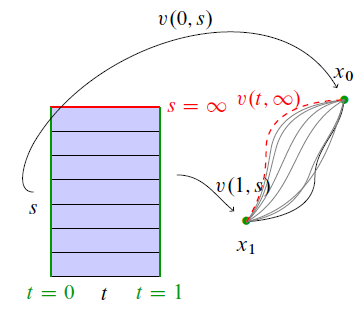
\includegraphics[scale=.45]{procedure.png}}
\caption{An Illustration of the Explicit Iterative Procedure to Solve the GHF \cite{PAPER1}}
\label{fig}
\end{figure}

The curves $v(t, \cdot):[0,1] \rightarrow \mathbb{R}^{n}$ act as the state-variable, and $s$ as the time-variable for the curve evolution. For large values of $k$, one can observe that the solution $v(t, \infty)$ tends to an admissible curve joining $v_{0}$ to $v_{1}$ \cite{PAPER1}, that is
\begin{equation}
\frac{d}{d t} v(t, \infty) \in \Delta_{0}(v(t, \infty))
\end{equation}

Finally, one can obtain the controls from the admissible curve $v(t, \infty)$ using

\begin{equation}
\left(\begin{array}{c}
u_{1}(t) \\
u_{2}(t) \\
\vdots \\
u_{p}(t)
\end{array}\right)=F_{p}^{\dagger}(v(t)) \dot{v}(t)
\end{equation}

\section{\textbf{Implementation and Results}}
\subsection{Benchmark Example}

The main goal of this case study is to demonstrate that the proposed novelty method works for a benchmark example and to extend it to an application of interest. The benchmark example considers a two link planar arm which has 2 degrees of freedom being the joint angles $(\theta_1, \theta_2)$. The actuators are servo drives which are located on the joints. The motors apply a certain commanded torque that rotates the joint which results in the motion of the end-effector. The motion planning problem for this particular case aims to figure out an admissible sequence of controls to steer the end-effector of the robot from an initial state $x_i$ to a final state $x_f$. The holonomic constraints that describe the dynamics of the motion is of the subsequent form:
 
\begin{equation}
\begin{aligned}
&q_{1}(x)= L_{1} \cos \left(\theta_{1}\right)+L_{2} \cos \left(\theta_{2}\right)-x=0 \\
&q_{2}(x)= L_{1} \sin \left(\theta_{1}\right)+L_{2} \sin \left(\theta_{2}\right)-y=0
\end{aligned}
\end{equation}
\\
where $L_{1}$ and $L_{2}$ are assumed to be $1$. By taking the differential of the two constraints, one obtains

\begin{equation}
\begin{aligned}
&\frac{\partial q_{1}}{\partial x}=\left(-1,0,-L_{1} \sin \theta_{1}, L_{2} \sin \theta_{2}\right)^{\top} \\ 
&\frac{\partial q_{2}}{\partial x}=\left(0,-1, L_{1} \cos \theta_{1}, L_{2} \cos \theta_{2}\right)^{\top}
\end{aligned}
\end{equation}
\\
to form the $F_c$ and $F_f$ matrices where $F_{f}(x)^{\top} F_{c}(x)=0$ is satisfied.

\begin{equation}
\resizebox{0.45\hsize}{!}{%
F_{c} = \left(\begin{array}{cc}1 & 0 \\ 0 & 1 \\ \sin \theta_{1} & -\cos \theta_{1} \\ \sin \theta_{2} & -\cos \theta_{2}\end{array}\right)}, \; \; %
\resizebox{0.45\hsize}{!}{%
F_{f}=\left(\begin{array}{cc}-\sin \theta_{1} & -\sin \theta_{2} \\ \cos \theta_{1} & \cos \theta_{2} \\ 1 & 0 \\ 0 & 1\end{array}\right)}
\end{equation}
\\*
Using $G(x) = F(x) D F^{\top}(x)$ yields
\\
\\
\hspace*{-1cm}
\resizebox{1.25\hsize}{!}{%
\begin{equation}
\renewcommand*{\arraystretch}{1.5}
G(x) = \left(\begin{array}{cccc}
\sin ^{2} \theta_{1}+\sin ^{2} \theta_{2}+k & -\frac{\sin 2 \theta_{1}}{2}-\frac{\sin 2 \theta_{2}}{2} & (k-1) \sin \theta_{1} & (k-1) \sin \theta_{2} \\
-\frac{\sin 2 \theta_{1}}{2}-\frac{\sin 2 \theta_{2}}{2} & \cos ^{2} \theta_{1}+\cos ^{2} \theta_{2}+k & -(k-1) \cos \theta_{1} & -(k-1) \cos \theta_{2} \\
(k-1) \sin \theta_{1} & -(k-1) \cos \theta_{1} & k+1 & k \cos \left(\theta_{1}-\theta_{2}\right) \\ (k-1) \sin \theta_{2} & -(k-1) \cos \theta_{2} & k \cos \theta_{1}-\theta_{2} & k+1
\end{array}\right)
\end{equation}
}
\\
\\
\\
where $k = 300$. Later, the above defined geometric heat flow equation is solved using the pdepe function in MATLAB. The curve and the time interval is discretized with 250 points, initial and boundary conditions are set in separate functions. The simulation was executed for a total time of 4 seconds. Here are the initial and boundary conditions for the benchmark example exhibited in the table below.

\begin{table}[h!]
    \begin{center}
    \label{tab:table1}
    \begin{tabular}{|c|c|c|c|}
    	\hline
        \multicolumn{4}{|c|}{Boundary Condition - Initial}     \\ 
        \hline
        \textbf{$x$} & \textbf{$y$} & \textbf{$\theta_1$} & \textbf{$\theta_2$}\\
        \hline
        $\frac{\sqrt{2}}{2}$ & 1 - $\frac{\sqrt{2}}{2}$ & $\frac{\pi}{2}$ & $\frac{-\pi}{4}$ \\
        \hline
        \multicolumn{4}{|c|}{Boundary Condition - Final}       \\ 
        \hline
        \textbf{$x$} & \textbf{$y$} & \textbf{$\theta_1$} & \textbf{$\theta_2$}\\
        \hline
        $\frac{\sqrt{2}}{2}$ & $1 + \frac{\sqrt{2}}{2}$ & $\frac{\pi}{2}$ & $\frac{\pi}{4}$  \\
        \hline
        \multicolumn{4}{|c|}{Initial Condition}                \\ 
        \hline
        \textbf{$x$} & \textbf{$y$} & \textbf{$\theta_1$} & \textbf{$\theta_2$}\\
        \hline
        $\frac{\sqrt{2}}{2}$ & $1 - \frac{\sqrt{2}}{2} + (\sqrt{2}t)$ & $\frac{\pi}{2}$ &  $-\frac{\pi}{4} + (\frac{\pi}{2}t)$							 \\
        \hline
    \end{tabular}
    \captionsetup{justification=centering}
    \caption{Table of Initial and Boundary Conditions \\ for the Benchmark Example}
    \end{center}
\end{table}
\\*
The comparison of the target and the actual path is illustrated in the successive figures.

{\centering
\begin{figure}[htbp]
\captionsetup{justification=centering}
\centerline{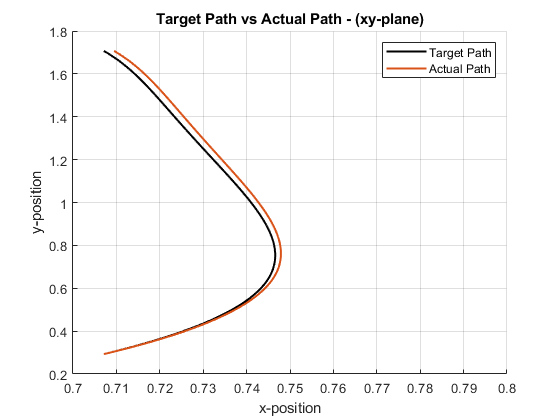
\includegraphics[scale=.475]{results_1_1.png}}
\caption{Results for the Benchmark Example ($xy$-plane)}
\label{fig}
\end{figure}
\\
\begin{figure}[htbp]
\captionsetup{justification=centering}
\centerline{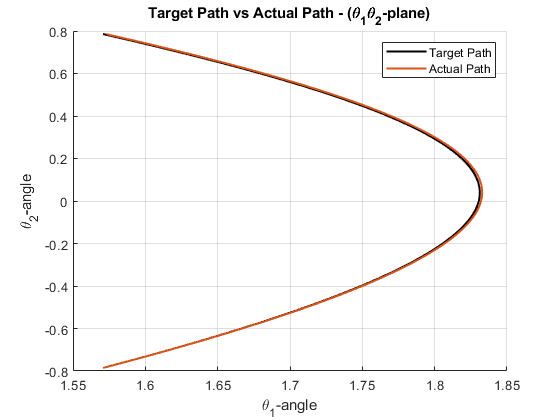
\includegraphics[scale=.475]{results_1_2.png}}
\caption{Results for the Benchmark Example ($\theta_{1}\theta_{2}$-plane)}
\label{fig}
\end{figure}
}

The difference between the target path and the actual path $v(t, \infty)$ decreases as $s$ increases. Additionally, the error diminishes as the number of points set to describe a curve $v(t, \cdot)$ rises. As this implementation considers finite discretization points and $s$, the actual and the target path differ. 

\newpage

\subsection{Two-link Planar Arm with Additional Holonomic Path Constraints}

The application of interest for this case study was to implement additional path constraints
for the benchmark example. Two constraints on the path $(q_3,q_4)$ were considered separately which restrict the motion of the end-effector to be vertical and circular respectively. The constraints are

\begin{equation}
\begin{aligned}
&q_{3}(x)= x - x_i = 0 \\
&q_{4}(x)= (x - x_c)^2 + (x - y_c)^2 - r^2 = 0
\end{aligned}
\end{equation}
\\

where $(x_c, y_c, r) =  (0, 1, 1)$. The differentials yield

\begin{equation}
\begin{aligned}
&\frac{\partial q_{3}}{\partial x}=\left(1, 0, 0, 0\right)^{\top} \\ 
&\frac{\partial q_{4}}{\partial x}=\left(2x, \; 2y - 2, \; 0, \; 0\right)^{\top}
\end{aligned}
\end{equation}
\\

Abiding by the process, $F_c$, $F_f$, matrices are attained to compute the $G$ matrix for each case. Due to their size, these matrices are too large to be explicitly written out. Their derivation will be present in the uploaded material. The same initial and boundary conditions as in the benchmark example were used for each of the cases.

{\centering
\begin{figure}[htbp]
\captionsetup{justification=centering}
\centerline{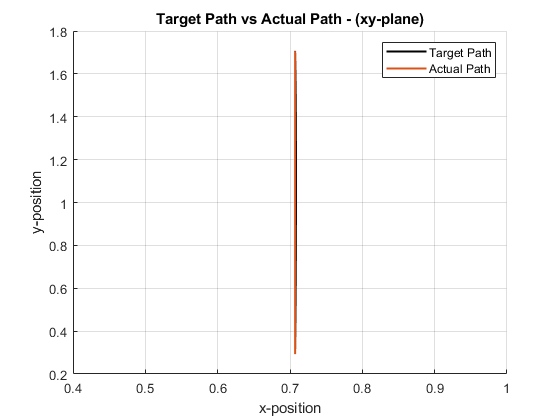
\includegraphics[scale=.475]{results_2_1.png}}
\caption{Results for the Vertical Motion Example ($xy$-plane)}
\label{fig}
\end{figure}
\\
\begin{figure}[htbp]
\captionsetup{justification=centering}
\centerline{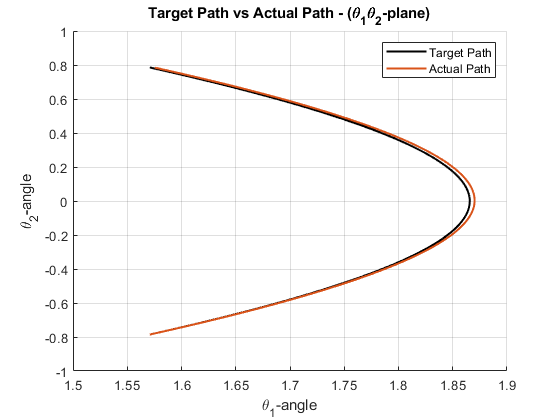
\includegraphics[scale=.475]{results_2_2.png}}
\caption{Results for the Vertical Motion Example ($\theta_{1}\theta_{2}$-plane)}
\label{fig}
\end{figure}
}

{\centering
\begin{figure}[htbp]
\captionsetup{justification=centering}
\centerline{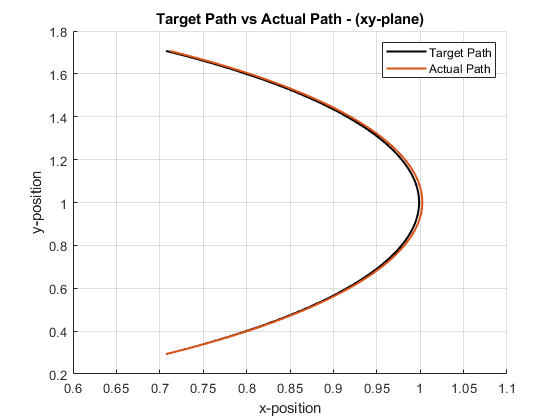
\includegraphics[scale=.475]{results_3_1.png}}
\caption{Results for the Circular Motion Example ($xy$-plane)}
\label{fig}
\end{figure}
\\
\begin{figure}[htbp]
\captionsetup{justification=centering}
\centerline{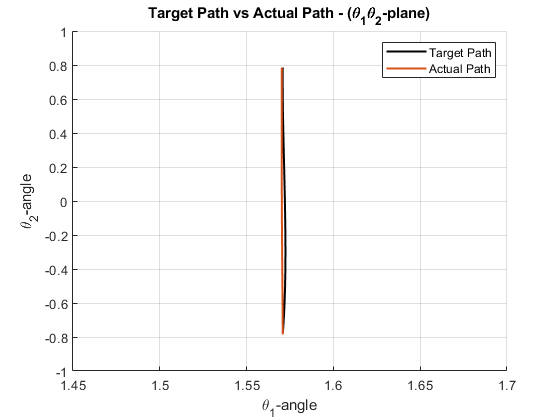
\includegraphics[scale=.475]{results_3_2.png}}
\caption{Results for the Circular Motion Example ($\theta_{1}\theta_{2}$-plane)}
\label{fig}
\end{figure}
}

The error magnitudes are presented in Table II.

\begin{table}[h!]
    \begin{center}
    \label{tab:table1}
    \begin{tabular}{|c|c|c|c|c|}
    	\hline
        \multicolumn{5}{|c|}{Average Error of the Actual Path}     \\ 
        \hline
        Case & \textbf{$x$} & \textbf{$y$} & \textbf{$\theta_1$} & \textbf{$\theta_2$}\\
        \hline
        Benchmark & 3.2 \cdot 10^{-4} & 4.3 \cdot 10^{-3} & 3.7 \cdot 10^{-3} & 6.3 \cdot 10^{-4} \\
        \hline
        Vertical Motion & 4.1 \cdot 10^{-4} & 4.4 \cdot 10^{-3} & 3.8 \cdot 10^{-3} & 7.2 \cdot 10^{-4} \\
        \hline
        Circular Motion & 2.5 \cdot 10^{-4} & 4.2 \cdot 10^{-3} & 3.7 \cdot 10^{-3} & 5.6 \cdot 10^{-4}\\
        \hline
    \end{tabular}
    \captionsetup{justification=centering}
    \caption{Error Magnitudes}
    \end{center}
\end{table}

\section{\textbf{Conclusion}}

In this case study, a proposed novel method for motion planning of non-holonomic systems were discussed and summarized. The method termed MotionSketch was explained in detail with the underpinning PDE problem. As an extension to the work of M. Belabbas  and S. Liu \cite{PAPER1}, \cite{PAPER2} the technique was implemented with additional constraints for an application of interest. The results were illustrated in comparison and the viability of the method was shown with the similarity of error magnitudes. For further improvement of the results, discretization steps and the "time" variable $s$ can be increased \cite{PAPER1}. Future work could be done on how to implement additional non-holonomic or obstacle constraints.

\newpage
\section*{\textbf{Acknowledgement}}
This case study was done as a part of the Mathematical Simulation Techniques course at Technische Universität Dortmund. The guidance and the support of the instructor and the teaching assistants are acknowledged.

\bibliographystyle{IEEETran}
\begin{thebibliography}{8}

\bibitem{PAPER1}
Belabbas, Mohamed Ali, and Shenyu Liu. "New method for motion planning for non-holonomic systems using partial differential equations." 2017 American Control Conference (ACC). IEEE, 2017.

\bibitem{PAPER2}
Liu, Shenyu, and Mohamed Ali Belabbas. "A homotopy method for motion planning." arXiv preprint arXiv:1901.10094 (2019).

\bibitem{AI1}
Latombe, Jean-Claude. Robot motion planning. Vol. 124. Springer Science & Business Media, 2012.

\bibitem{AI2}
Zhang, Jian. "AI based Algorithms of Path Planning, Navigation and Control for Mobile Ground Robots and UAVs." arXiv preprint arXiv:2110.00910 (2021).

\bibitem{OC1}
Schultz, Jarvis, Elliot Johnson, and Todd D. Murphey. "Trajectory optimization in discrete mechanics." Differential-Geometric Methods in Computational Multibody System Dynamics. Springer International Publishing (2015).

\bibitem{OC2}
C. R. Hargraves and S. W. Paris, "Direct Trajectory Optimization Using Nonlinear Programming and Collocation", Journal of Guidance, Control, and Dynamics, vol. 10, no. 4, pp. 338–342, 1987.

\bibitem{MATH1}
Hargraves, Charles R., and Stephen W. Paris. "Direct trajectory optimization using nonlinear programming and collocation." Journal of guidance, control, and dynamics 10.4 (1987): 338-342.

\bibitem{MATH2}
Brockett, Roger W., and Liyi Dai. "Non-holonomic kinematics and the role of elliptic functions in constructive controllability." Nonholonomic motion planning. Springer, Boston, MA, 1993. 1-21.

\bibitem{MATH3}
Laumond, Jean-Paul, ed. Robot motion planning and control. Vol. 229. Berlin: Springer, 1998.

\bibitem{PRM}
Kavraki, Lydia E., et al. "Probabilistic roadmaps for path planning in high-dimensional configuration spaces." IEEE transactions on Robotics and Automation 12.4 (1996): 566-580.

\bibitem{GRAPH}
Chen, Pang C., and Yong K. Hwang. "SANDROS: a dynamic graph search algorithm for motion planning." IEEE Transactions on Robotics and Automation 14.3 (1998): 390-403.

\bibitem{APF}
Khatib, Oussama. "Real-time obstacle avoidance for manipulators and mobile robots." Autonomous robot vehicles. Springer, New York, NY, 1986. 396-404.

\bibitem{MATH4}
Jost, Jürgen, and Jèurgen Jost. Riemannian geometry and geometric analysis. Vol. 42005. Berlin: Springer, 2008.

\end{thebibliography}

\end{document}
